\begin{figure}[htpb]
	\centering\capstart{}
	\subfloat[Cheetah
			(\(\num{2002}\, \mathcal{V}\))]
	{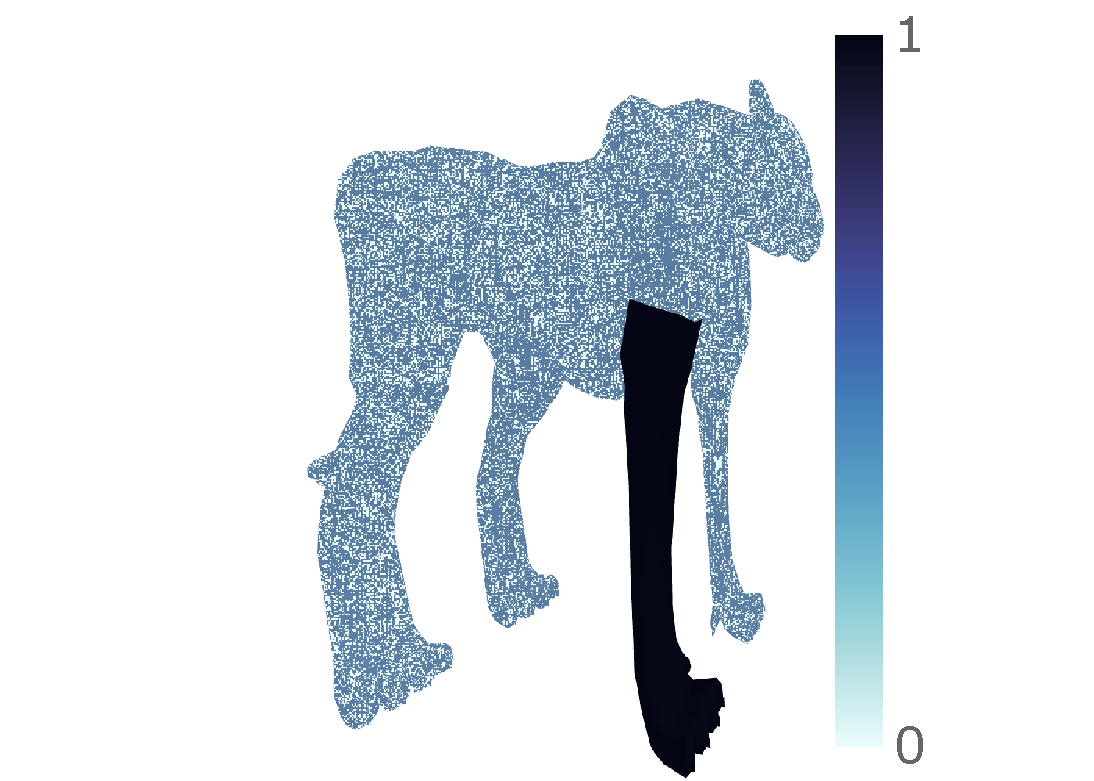
\includegraphics[trim={137 1 3 7},clip,width=.28\textwidth]{cheetah_region_norm.pdf}}
	\hfill
	\subfloat[Dragon
			(\(\num{1166}\, \mathcal{V}\))]
	{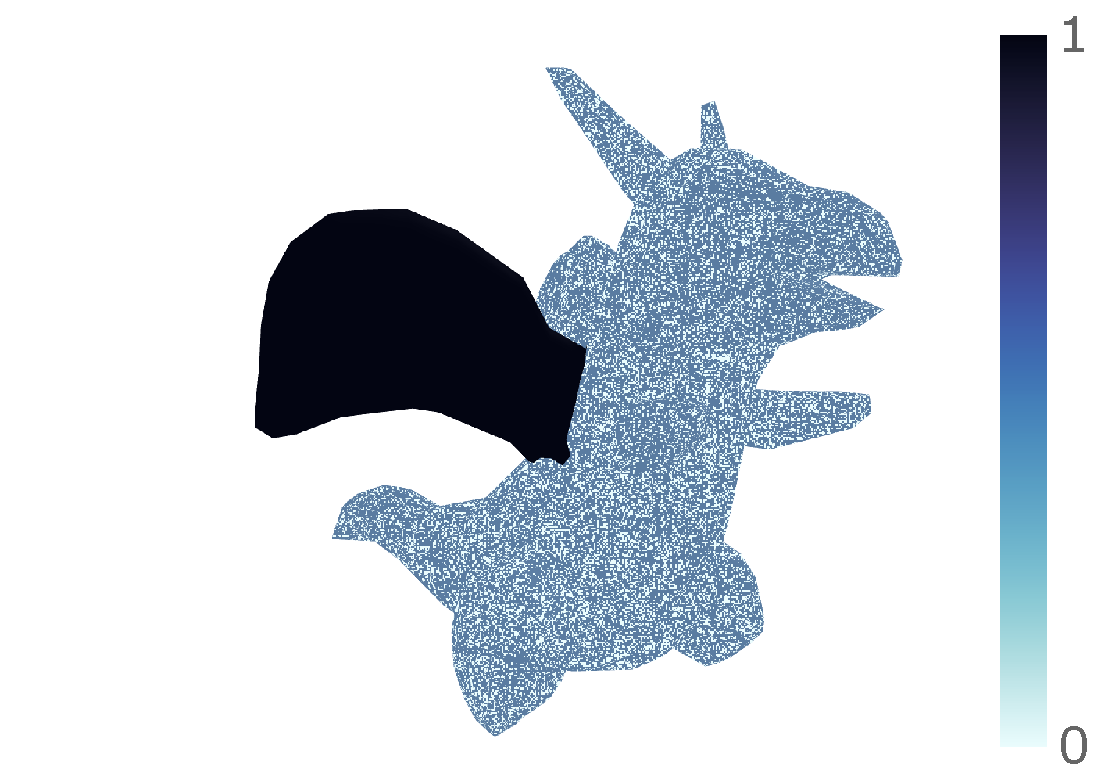
\includegraphics[trim={75 8 3 7},clip,width=.33\textwidth]{dragon_region_norm.pdf}}
	\hfill
	\subfloat[Bird
			(\(\num{699}\, \mathcal{V}\))]
	{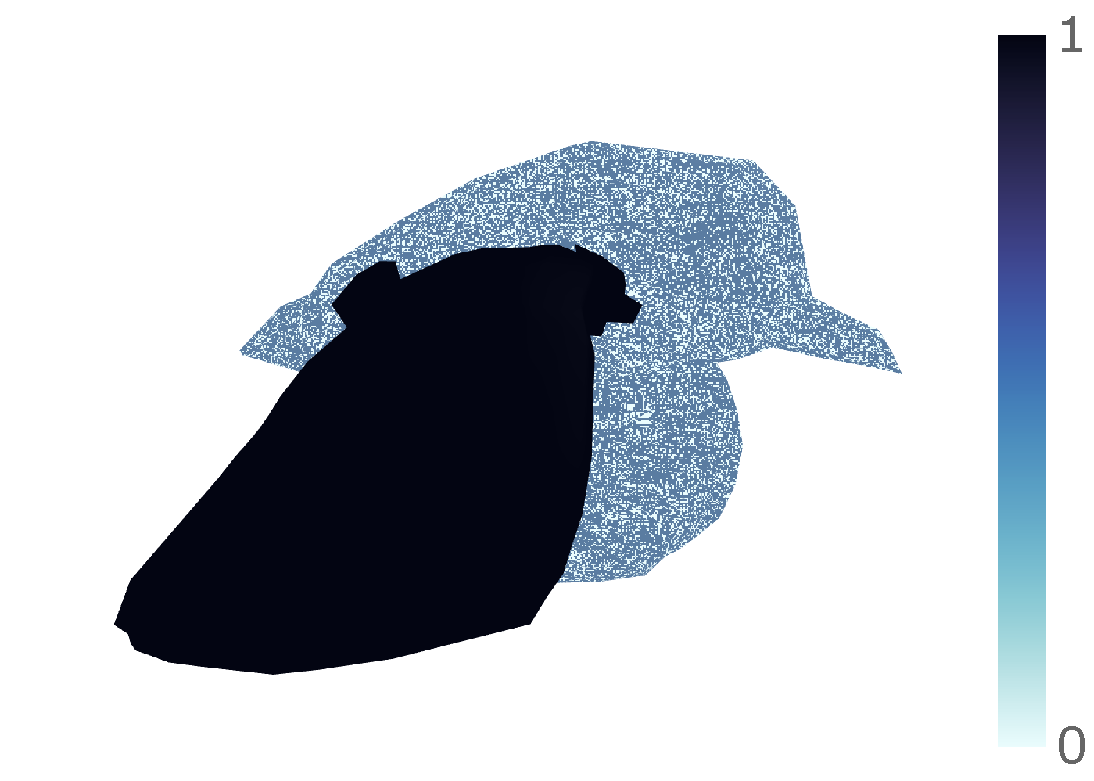
\includegraphics[trim={7 8 3 7},clip,width=.38\textwidth]{bird_region_norm.pdf}}
	\newline
	\subfloat[Teapot
			(\(\num{726}\, \mathcal{V}\))]
	{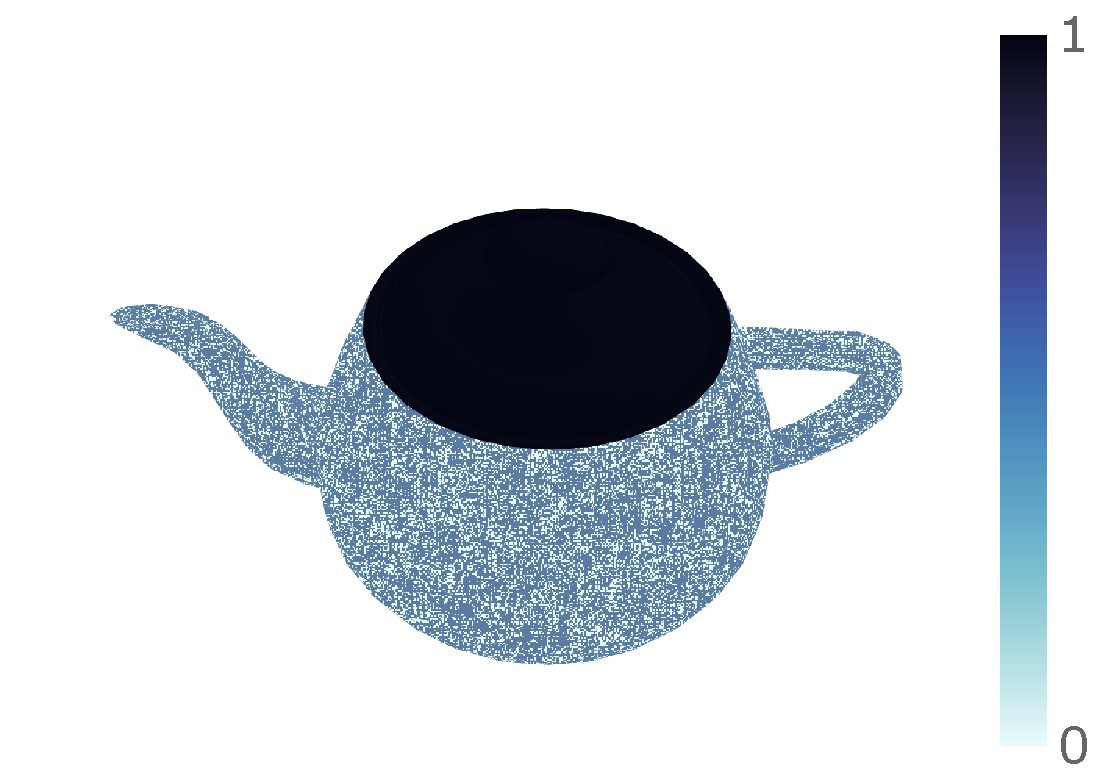
\includegraphics[trim={3 8 3 7},clip,width=.37\textwidth]{teapot_region_norm.pdf}}
	%
	\subfloat[Cube
			(\(\num{6146}\, \mathcal{V}\))]
	{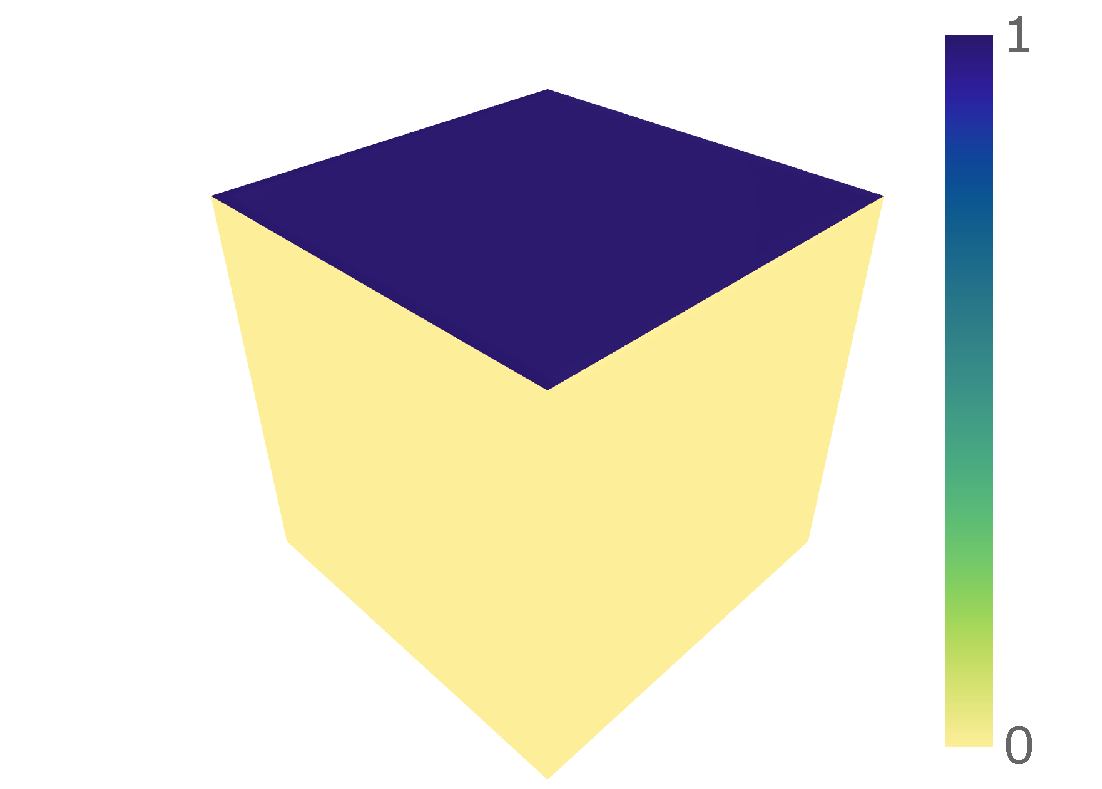
\includegraphics[trim={62 1 3 7},clip,width=.33\textwidth]{cube_region_norm.pdf}}
	\caption[
		The Slepian regions of some other meshes used in denoising
	]{
		The Slepian regions (in blue) and the corresponding number of vertices \(\vertices{}\) of some other meshes.
		The same denoising procedure as in \cref{fig:chapter4_denoising} was performed for these alternative meshes, the results of which are shown in \cref{tab:chapter4_denoising}.
	}\label{fig:chapter4_other_meshes}
\end{figure}
